% =====================================================================
%  Companion-Praesentation zum A1-Poster (Pan/Zoom-Stil)
%
%  Alle Seiten haben dieselbe Groesse (A1 hochkant). Auf jeder Seite wird
%  das komplette Poster skaliert und so verschoben, dass die jeweilige
%  Zielregion in der Mitte landet -- der Rest des Plakats laeuft an den
%  Raendern weiter sichtbar.
%
%  Reihenfolge:
%    1. Uebersicht  (skalierung 1, ganzes Poster)
%    2. Einstieg
%    3. Toolchain
%    4. Zwischenstand
%    5. Wichtigste Quelle
%    6. Zeitplan
%
%  Vor dem Bauen muss poster.pdf vorliegen.
%  A1 = 594 x 841 mm. Plakatmitte = (297, 420.5).
% =====================================================================
\documentclass{article}
\usepackage[paperwidth=594mm, paperheight=841mm, margin=0mm]{geometry}
\usepackage{graphicx}
\usepackage{tikz}

\pagestyle{empty}
\setlength{\parindent}{0pt}

% ----------------------------------------------------------------------
%  \zoomslide{cx}{cy}{scale}
%    cx, cy  = Mittelpunkt der Zielregion auf dem Poster
%              (mm, gemessen von OBEN-LINKS)
%    scale   = Zoomfaktor (1.0 = ganzes Poster)
%
%  Das Poster wird als skaliertes Bild platziert und so verschoben, dass
%  der Punkt (cx, cy) auf der Seitenmitte (297, 420.5) liegt.
%  Bereiche, die ueber den Seitenrand hinausragen, werden vom PDF-Viewer
%  abgeschnitten.
% ----------------------------------------------------------------------
\newcommand{\zoomslide}[3]{%
  \begin{tikzpicture}[remember picture, overlay]
    \pgfmathsetmacro{\sxmm}{(297-#1)*#3}%
    \pgfmathsetmacro{\symm}{(#2-420.5)*#3}%
    \node[inner sep=0, scale=#3]
      at ([xshift=\sxmm mm, yshift=\symm mm] current page.center)
      {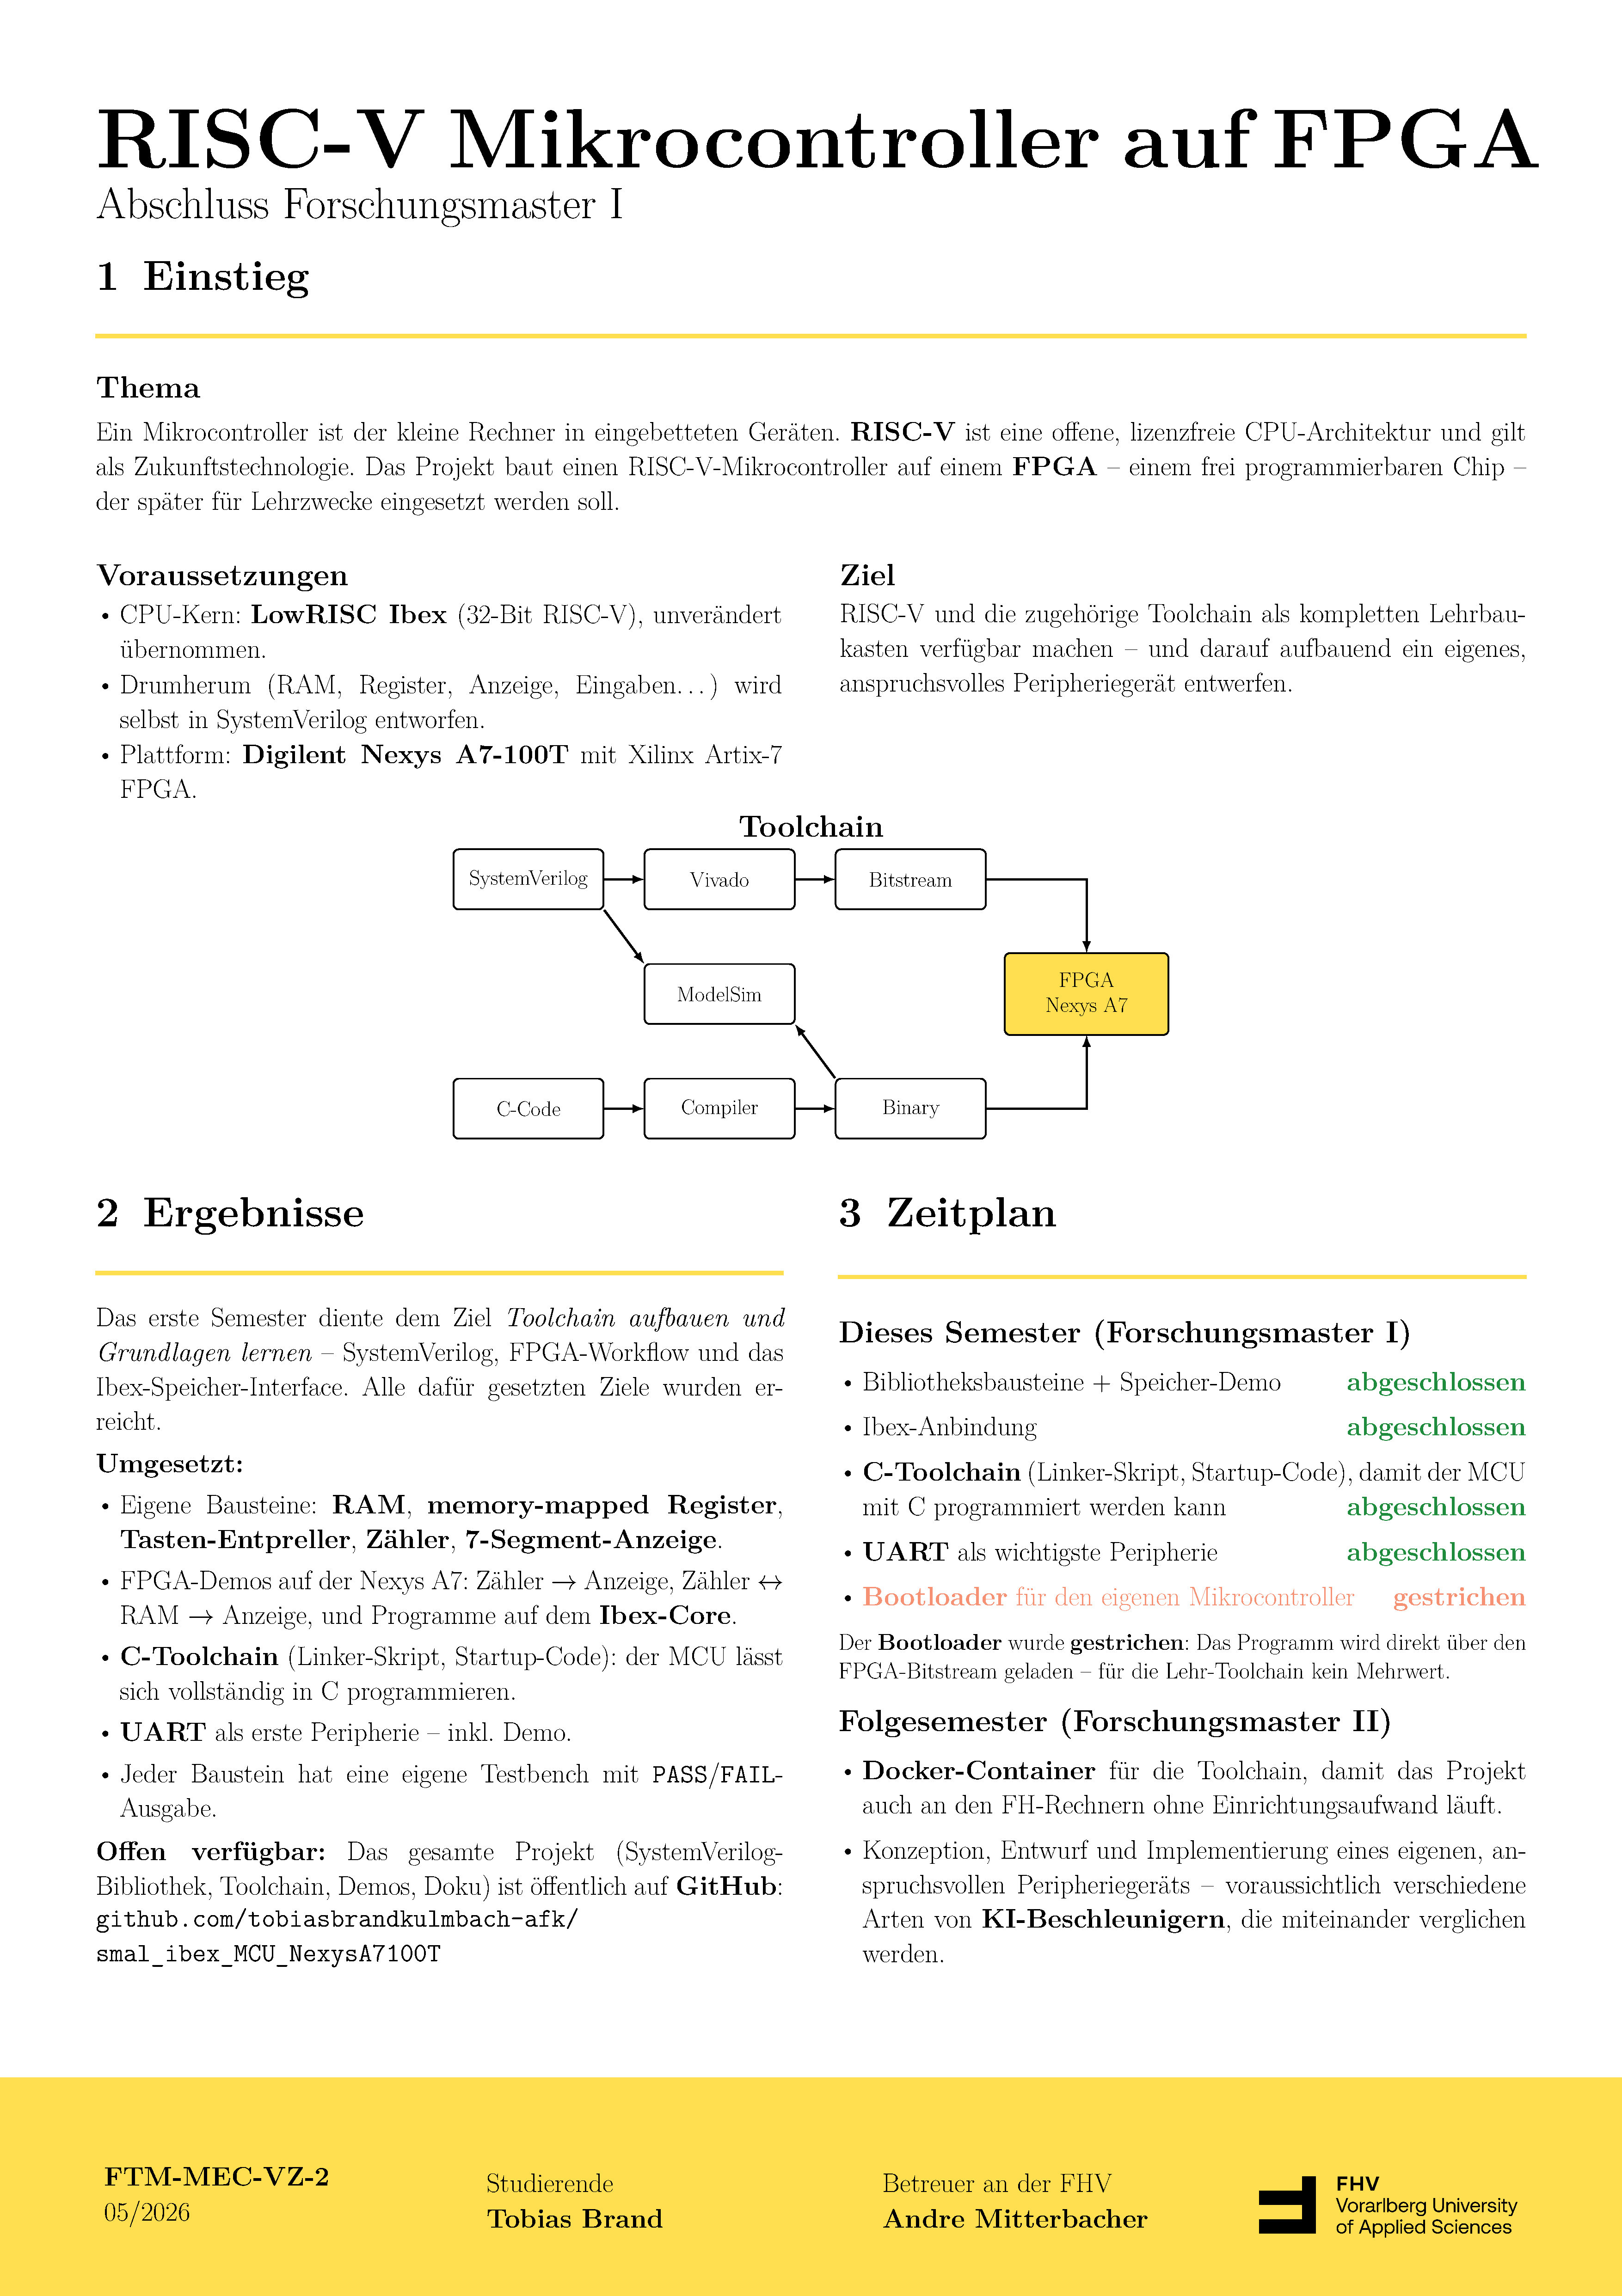
\includegraphics[width=594mm]{poster.pdf}};
  \end{tikzpicture}%
  \clearpage
}

\begin{document}

% Damit die erste Seite tatsaechlich erzeugt wird, brauchen wir minimal
% etwas Inhalt -- der TikZ-Overlay liefert das.

% ---------- 1. Uebersicht (volles Poster, kein Zoom) ------------------
\zoomslide{297}{420.5}{1.0}

% ---------- 2. Einstieg (Titel + Thema + Voraus + Ziel) ---------------
% Region etwa y = 0..316 mm, volle Breite -> Mitte (297, 158)
\zoomslide{160}{270}{2}

\zoomslide{430}{270}{2}

% ---------- 3. Toolchain (Heading + Flowchart) ------------------------
% Region etwa y = 320..446 mm, volle Breite -> Mitte (297, 383)
\zoomslide{297}{380}{2}

% ---------- 4. Zwischenstand (linke Spalte) ---------------------------
% Region etwa x = 15..300, y = 400..640 -> Mitte (157, 520)
\zoomslide{160}{600}{2}

% ---------- 6. Zeitplan (rechte Spalte) -------------------------------
% Region etwa x = 300..579, y = 400..720 -> Mitte (439, 560)
\zoomslide{430}{600}{2}

\zoomslide{297}{420.5}{1}

\end{document}
